\documentclass{report}
\usepackage[utf8]{inputenc}
\usepackage{graphicx}

\begin{document}

\subsection{Experiment four}
\textbf{Ticktime influence on the Blacklist algorithm with a fixed cluster fail-over pattern using a random sample size}
\\~\\
The same heartbeat rate is used from experiment one. The same random sample size from experiment three will be used. For this experiment the first cluster of four raspberry pi's will be disabled at heartbeat 3.000. After that every 2.000 heartbeats an additional cluster will be disabled until there is only one cluster left. A flowchart can be found in figure ~\ref{fig:FlowChart4}.

\begin{figure}[htb]
	\centering
	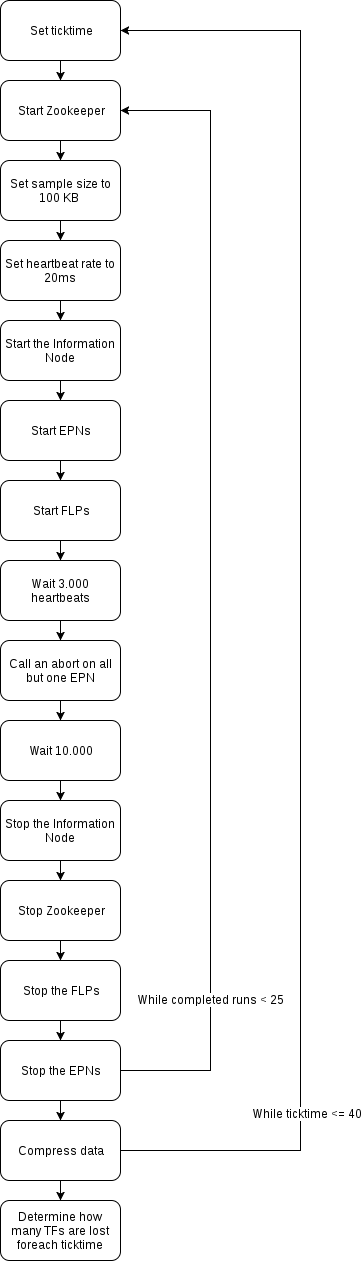
\includegraphics[scale=0.3]{./graphics/ex4.png}
	\caption{Flow chart experiment four}
	\label{fig:FlowChart4}
\end{figure}

\subsection{Experiment five}
\textbf{Ticktime influence on the Blacklist algorithm with a random cluster fail-over pattern using a random sample size}
\\~\\
The same heartbeat rate is used from experiment one. The same random sample size from experiment three will be used. For this experiment a random set of four raspberry pi's will be disabled at heartbeat 3.000. After that, every 2.000 heartbeats an additional set of four pi's will be disabled until there is only one set left. A flowchart can be found in figure ~\ref{fig:FlowChart5}.

\begin{figure}[htb]
	\centering
	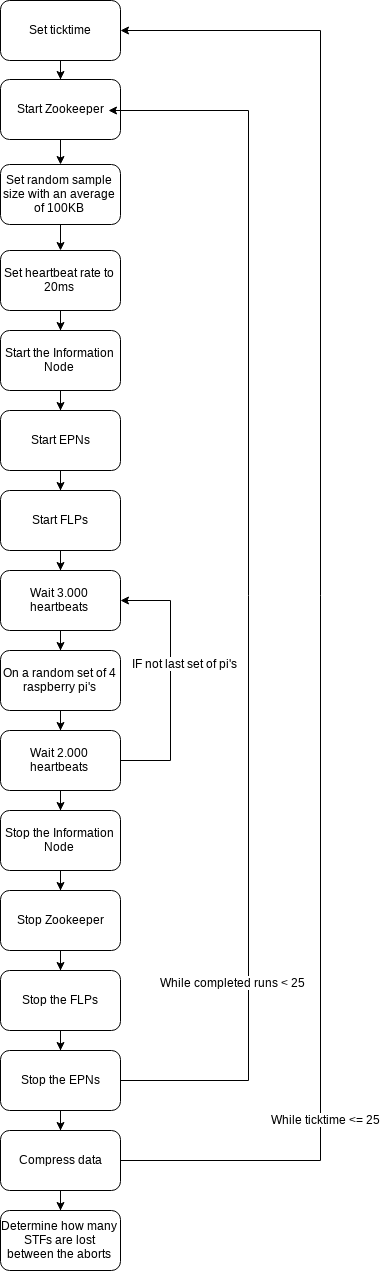
\includegraphics[scale=0.3]{./graphics/ex5.png}
	\caption{Flow chart experiment five}
	\label{fig:FlowChart5}
\end{figure}

\end{document}